% This text is proprietary.
% It's a part of presentation made by myself.
% It may not used commercial.
% The noncommercial use such as private and study is free
% Sep. 2005 
% Author: Sascha Frank 
% University Freiburg 
% www.informatik.uni-freiburg.de/~frank/



\pdfminorversion=5
\pdfobjcompresslevel=3 
\pdfcompresslevel=9

% Full presentation (with overlays, animated bullet items etc)
\documentclass[xcolor={x11names,svgnames,dvipsnames}]{beamer}

% Transparency mode (no overlays)
%\documentclass[xcolor={x11names,svgnames,dvipsnames},trans]{beamer}

% 4-up handout mode
%\documentclass[xcolor={x11names,svgnames,dvipsnames},handout]{beamer}
\usepackage{listings}

\usepackage{pgfpages}

\usepackage[british]{babel}
\usepackage{etex}

%% Glossy pretty look for the presentation and transparency (w/o overlays and animations) versions!
\mode<beamer|trans>{
	\useoutertheme[glossy]{wuerzburg}
	\useinnertheme[shadow,outline]{chamfered}
	\usecolortheme{shark}
}
\setbeamertemplate{navigation symbols}{}
\setbeamertemplate{frametitle continuation}[from second][(cont'd)]
\usefonttheme[stillsansseriftext,stillsansserifsmall]{serif}

%% Save up on ink for the 4-up handouts
\mode<handout>{
	\useoutertheme{wuerzburg}
	\useinnertheme[outline]{chamfered}
	\pgfpagesuselayout{4 on 1}[a4paper, landscape, border shrink=10mm]
	\pgfpageslogicalpageoptions{1}{border code=\pgfstroke}
	\pgfpageslogicalpageoptions{2}{border code=\pgfstroke}
	\pgfpageslogicalpageoptions{3}{border code=\pgfstroke}
	\pgfpageslogicalpageoptions{4}{border code=\pgfstroke}
}

\mode<presentation>{\AtBeginSection{%
		\begin{frame}
			\frametitle{Contents}
			\tableofcontents[currentsection]
		\end{frame}}}
		
		\usepackage{microtype}
		\usepackage[utf8]{inputenc}
		\usepackage[T1]{fontenc}
		\usepackage[osfss]{libertine}
		\usepackage[scaled=.77]{beramono}
		\usepackage{cmap}
		
		\usepackage{relsize,tabularx}
		\usepackage[T1,safe]{tipa}
		\usepackage{dtklogos,hologo,textcomp}
		\usepackage{multicol,booktabs}
		\usepackage{listings}
		\lstset{upquote,keepspaces=true,columns=spaceflexible,
			basicstyle=\ttfamily\scriptsize,%
			breaklines=true,breakindent=0pt,xleftmargin=0pt, xrightmargin=6pt,%
			language=[LaTeX]TeX, texcsstyle=*\bfseries\color{Maroon}, commentstyle=\sffamily\itshape\smaller\color{SeaGreen4},
			emphstyle=\bfseries\color{RoyalBlue3},escapechar={:},
			emphstyle={[2]{\bfseries\color{Sienna2}}},
			postbreak=\mbox{{\smaller\color{gray}$\hookrightarrow$}}
		}
		
		\usepackage{tikz}
		\usetikzlibrary{shapes,arrows,positioning,matrix,chains,backgrounds,fit}
		
		\usepackage{multicol}
		\usepackage[version=3]{mhchem}
		\usepackage{chemfig}
		\usepackage{linguex,qtree}
		\let\fg\lingfg
		\usepackage{texshade}
		\usepackage[detect-all]{siunitx}
		\usepackage[siunitx]{circuitikz}
		\usepackage{bytefield}
		\usepackage{auto-pst-pdf}
		\usepackage{pstricks,pst-barcode}
		\usepackage{pgfplots}
		\usepackage{pgfgantt}
		\usepackage[skaknew]{chessboard,skak}
		\usepackage{cwpuzzle}
		\usepackage{gchords,guitar}
		\usepackage{spreadtab}
		\usepackage{ccicons}


\setlength\fboxsep{0pt}
\SetTracking{encoding=*}{-39}

\author[\textsc{Jian} Wang]{\textsc{Jian} Wang\\[1ex]%
{\small\url{wangjian790@gmail.com}\\[-.5ex]\url{}}\\
{\small{Financial math Ph.D.}}\\
{\small{Florida State University}}\\
[0.8ex]\copyright\copyright\copyright\copyright} %\ccbyncsa}

\title{Option Pricing with Cuda Programming}
%\titlegraphic{\ccbyncsa}
\date[\textsc{PPT} 2018]{}%

% Include QR code of slides URL for presentation-mode only -- so that audience
%  can snap it and download it on the spot
\mode<beamer>{\titlegraphic{\begin{pspicture}\psbarcode[scalex=.75,scaley=.75]{http://liantze.penguinattack.org/latextypesetting.html\#mosc11-slides}{eclevel=L}{qrcode}\end{pspicture}}}

\hypersetup{%
pdfauthor={Jian Wang}, %% the "author" field from above includes garbage code...
pdfkeywords={HFC,Machine Learning,general}
}
\begin{document}
\begin{frame}
\maketitle
\end{frame}

%\title{Simple Beamer Class}   
%\author{Sascha Frank} 
%\date{\today} 

\frame{\frametitle{Table of contents}\tableofcontents} 

\section{Introduction to the GPU architecture}
\begin{frame}
\frametitle{GPU-Computing}
\begin{itemize}
 \item \textbf{GPU:} Graphicsx Processing Unit
\item \textbf{GPGPU}: General Purpose Graphics Processing Unit
\item \textbf{GPU-accelerated computing:} is the use of a GPU together with a CPU to accelerate scientific and engineering applications
\item \textbf{Remark}. GPU does NOT work by itself. It is used as a device of a CPU, and is often called “accelerator”
\item \textbf{Remark}. Intel call their Xeon Phi product “coprocessor”
\end{itemize}
 \begin{figure}
     
\includegraphics[width=0.8\textwidth, height=0.4\textheight]{intel.png}
\end{figure}
\end{frame}


\begin{frame}
\frametitle{GPU-Computing}
\begin{itemize}
 \item \textbf{Tegra:}
 mobile and embedded devices (e.g., smart phones)
 \item \textbf{GeForce:} consumer graphics (e.g., PC Gaming)
 \item \textbf{Quadro:} professional visualization (e.g., CAD)
 \item \textbf{Tesla:}
 parallel computing (what we have at RCC)
\end{itemize}
 \begin{figure}
     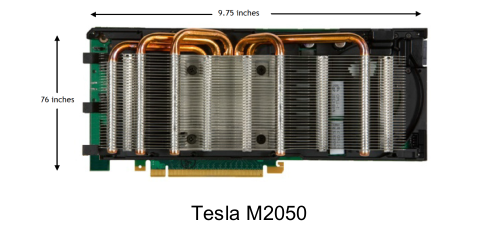
\includegraphics[width=0.8\textwidth, height=0.4\textheight]{tesla.png}
\end{figure}
\centering
{Tesla => Fermi => Kepler => Maxwell => Pascal
}

\end{frame}

\begin{frame}
\begin{itemize}
\item Tesla product family is classified using Compute Capability
\item Kepler class architecture has major version number 3
\item Fermi class architecture has major version number 2

\item Tesla class architecture has major version number 1
\end{itemize}
\begin{center}
\begin{tabular}{|c|c|}
\hline GPU & COMPUTE CAPABILITY \\ 
\hline Tesla K40  &  3.5\\ 
\hline Telsa K20 &  3.5\\ 
\hline  Telsa K10&  3.0\\ 
\hline  Telsa C2070&  2.0\\ 
\hline  Telsa C1060&  1.3\\ 
\hline 
\end{tabular}
\end{center}
 \centering{Telsa Family Compute Capability}
\end{frame}

\begin{frame}
\frametitle{Compute Capability}
\textbf{FERMI vs KEPLER}
\begin{center}
\begin{tabular}{|c|c|c|}
\hline  & FERMI  & KEPLER\\ 
  & (TESLA C2050)  & (TESLA k10)\\ 
\hline  CUDA Cores& 448  & 2 x 1536\\ 
\hline  Memory & 6 GB  & 8 GB\\ 
\hline  Peak Performance* & 1.03 Tflops  & 4.58 Tflops\\ 
\hline  Memory Bandwidth & 144 GB/s  & 320 GB/s\\ 
\hline
\end{tabular}
\end{center}
* Peak single- precision floating point performance 

\begin{itemize}
\item Question: are these many GPU cores equivalent to same
number of CPU cores?
\item Answer: no. (that would cost you a million dollars)
\end{itemize}

\end{frame}

\begin{frame}
\frametitle{GPU core VS CPU core}
\begin{itemize}
\item
\textbf{CPU core:} relatively heavy-weight, designed for complex
control logic, optimized for sequential programs.

\item
\textbf{GPU core:} relatively light-weight, designed with simple
control logic, optimized for data-parallel tasks, focusing on
throughput of parallel programs.

\item 
\textbf{CPU+GPU:} heterogeneous architecture
\end{itemize}

\end{frame}


\begin{frame}
\frametitle{Heterogenneous Architecture}
 \begin{figure}
     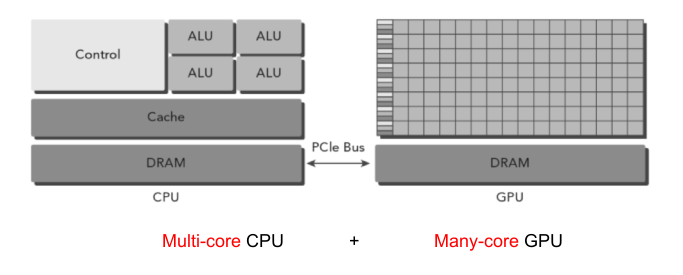
\includegraphics[width=0.8\textwidth, height=0.5\textheight]{gpu_architecture.png}
\end{figure}

\begin{itemize}
\item
\textbf{Remark:} GPU has its own memory, connect to CPU via PCI-express
bus
\item \textbf{Remark:} Differentiate Multi-Core from Many-Core (e.g., Intel Xeon Phi
co-processor is also many-core).

\end{itemize}

\end{frame}


\begin{frame}
\frametitle{CUDA Programming Model}
\textbf{Question:} how to use GPU to accelerate your code?
\begin{itemize}
\item A. Figure out which part of your code need speedup.
\item B. Rewrite that part of your program for GPU using CUDA.
\item C. Re-compile your program for GPU (nvcc -o a.out a.cu).
\item D. Send that piece of Code to GPU memory (automatic).
\item E Send the data needed to GPU memory (by you).
\item F. Copy the resulting data back to CPU memory (by you).
\item G. Continue your CPU calculation.

\end{itemize}

\end{frame}
\section {GPU/CUDA programming model}
\begin{frame}
\frametitle{CUDA Programming Model}
\begin{itemize}
\item Divide your code into Host (CPU) and Device (GPU) Code
\item Processing flow of a CUDA program:
\begin{itemize}
\item a. Copy data from CPU memory to GPU memory
\item b. Invoke kernel to run on the GPU.
\item c. Copy data back from GPU to CPU memory
\item  d. Release the GPU memory and reset the GPU.
\end{itemize}

\item CUDA code file name extension .cu
\item CUDA compiler: nvcc (it compiles .c, .cpp too!)

\item \$ nvcc -lm -o a.out a.cu
\end{itemize}

\end{frame}


\begin{frame}
 \begin{figure}
     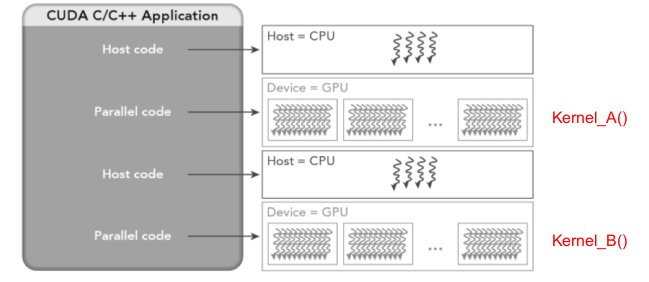
\includegraphics[width=0.8\textwidth, height=0.5\textheight]{kernel.png}
\end{figure}

\begin{itemize}
\item The kernel function run concurrently by many threads on the GPU.
\item CPU might or might not wait for GPU depending on synchronization.
(Q: when GPU is busy, what is CPU doing?)
\item You can have more than one kernel functions in your CUDA APP
\end{itemize}
\end{frame}

\begin{frame}
\frametitle{2-Level Thread Hierarchy (p1)}

\begin{itemize}
\item There are many many threads, so they need be managed.
\item Grid: All threads spawned by a single kernel.
\item  Grid is made up of many thread blocks.
\item A thread block is a group of threads which can cooperate\\
\ \	Intra-block synchronization\\
\ \	Sharing memory within a block\\
\ \	NO memory sharing or synchronization across blocks
\item 
A thread finds its own unique id using two coordinates:
blockIdx and threadIdx, for example (1D case):
\\
\ \ id = threadIdx.x + blockIdx.x*blockDim.x

\textbf{Summary:} Level 1 is a grid of blocks; level 2 is block of threads

\end{itemize}

\end{frame}


\begin{frame}
\frametitle{2-Level Thread Hierarchy}
 \begin{figure}
     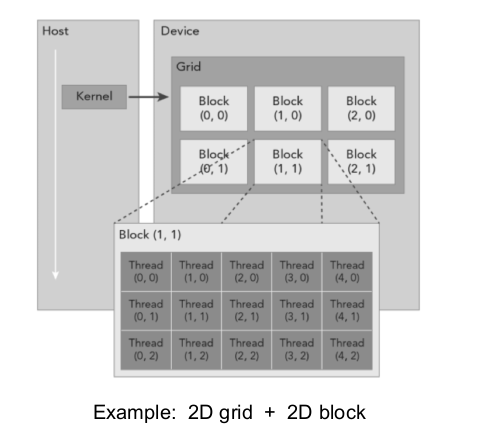
\includegraphics[width=0.9\textwidth, height=0.9\textheight]{kernel_2.png}
\end{figure}

\end{frame}

\begin{frame}
\begin{itemize}
\item Declaration Syntax:\\
\_\_global\_\_ void kernel(arg1, arg2, ...)\{\\
\ \ \ \ \ \ \  function body;\\
\}
\item  \_\_global\_\_ is a function type qualifier.
\item Kernel function is invoked by CPU, but run on GPU with
many copies (one thread per copy).
\item Kernel invoking Syntax:\\
\ \ kernel<<<grid, block>>>(arg1, arg2, ...)\\
\ \ both grid, block are of type dim3, e.g.,\\
\ \ dim3 gridDim(256,256,1); dim3 blockDim(16,16,1);\\
\end{itemize}
\end{frame}

\begin{frame}
\frametitle{CUDA Function Type Qualifiers}
Declaration Syntax:\\
\_\_global\_\_ void name1(arg1, arg2, ...)\{\\
\ \ \ \ name2(arg1,arg2); // invoke device function\\
\}\\
\_\_device\_\_ double name2(arg1, arg2, ...)\{\\
\ \ \ \ function body;\\
\}\\
\_\_host\_\_ float name3(arg1, arg2, ...)\{\\
\ \ \ \ function body;\\
\}\\
Host and device routines only run on CPU, and GPU respectively.
Global declares kernel function, run on GPU, which can call device
functions.

\end{frame}

\begin{frame}
\frametitle{CUDA Kernel Function}

\textbf{Question:} What should be put in the Kernel function?\\
for (i = 0; i < 1000; i++)\\
\ \ \ \ C[i] = A[i] + B[i];\\
\}\\

\_\_global\_\_ void kernel(int* A, int* B, int* C) \{\\
\ \ \ \ id = threadIdx.x + blockIdx.x*blockDim.x;\\
\ \ \ \ C[id] = A[id] +B[id];\\
\}\\
In essence, your for loop with for peeled off, but keep the
things inside.\\
The key part is to map your data to threads (array indices).

\end{frame}

\begin{frame}
\begin{itemize}
\item Question: How to move data between CPU and GPU?\\
\ \ \ \ cudaMalloc( (void**) A\_d, size\_t n\_bytes);\\
\ \ \ \ cudaMemcpy(ptr\_dest, ptr\_src, n\_bytes, direction);\\
\item Where\\
\ \ \ \ ptr\_dest, ptr\_src are destination/source pointers;\\
\ \ \ \ direction can be\\
\ \ \ \ \ \ \ \ cudaMemcpyHostToDevice\\
\ \ \ \ \ \ \ \ cudaMemcpyDeviceToHost\\
\ \ \ \ \ \ \ \ cudaMemcpyDeviceToDevice\\
\item How to free Cuda Memory?\\
\ \ \ \ cudaFree(A\_d);
\end{itemize}
\end{frame}

\begin{frame}
\frametitle{CUDA Memory Operations}
 \begin{figure}
     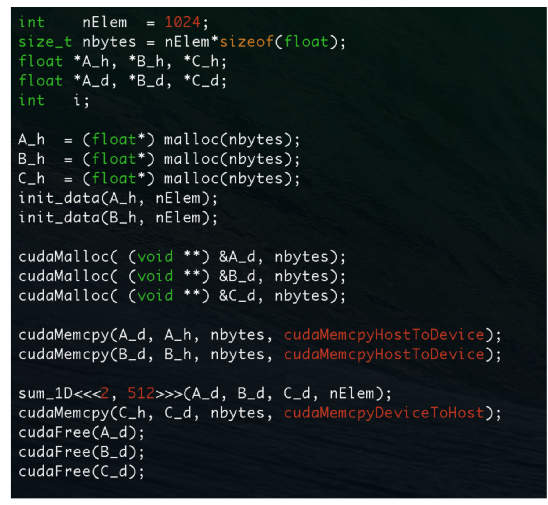
\includegraphics[width=0.8\textwidth, height=0.8\textheight]{code.png}
\end{figure}
\end{frame}

\begin{frame}
Example: Sum two 1D arrays assuming 1D block and 1D grid:
Here is the kernel routine sum\_1D:
 \begin{figure}
     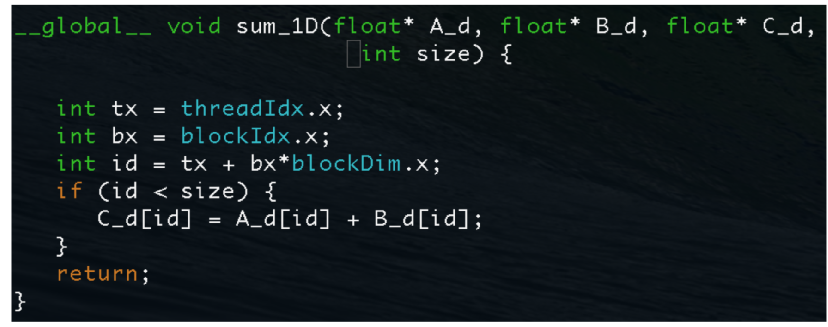
\includegraphics[width=0.8\textwidth, height=0.4\textheight]{code2.png}
\end{figure}
The main function was already shown in the previous page
 \begin{figure}
     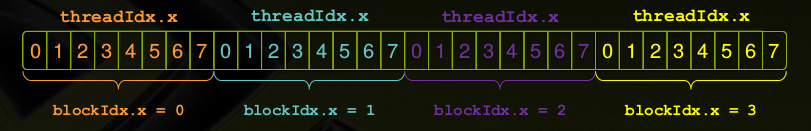
\includegraphics[width=0.8\textwidth, height=0.2\textheight]{thread.png}
\end{figure}

\end{frame}


\begin{frame}
\frametitle{How to Compile CUDA Code?}
Cuda nvcc compiler (cuda-7.0 at the RCC):\\
\\
\vspace{0.5cm}

a. Pure C code: a.c\\
\ \ \ \ \$ nvcc -o a.out a.c\\
\vspace{1cm}


b. Single Cuda code: a.cu\\
\ \ \ \ \$ nvcc -arch sm\_20 -O3 -o a.out a.cu\\
\vspace{1cm}


c.C and Cuda Mixed: a.cu and b.c\\
\ \ \ \ \$ gcc -o b.o -c b.c (or icc if you use intel compiler)\\
\ \ \ \ \$ nvcc -o a.out b.o a.cu\\
\end{frame}

\begin{frame}
\frametitle{Use GPU ON the HPC Cluster}


\begin{columns}
\column{2.4in}
Step 1: Load the cuda module\\
\ \ \ \ \$ module load cuda\\
\vspace{1cm}
Step 2: Compile your cuda code\\
\ \ \ \ \$ nvcc -o a.out a.cu\\
\vspace{1cm}
Step 3: Create a SLURM job script\\
\ \ \ \ \$ vi slurm.sub\\
\vspace{1cm}
Step 4: Submit your job.\\
\ \ \ \ \$sbatch slurm.sub
\column{2.5in}
 \begin{figure}
     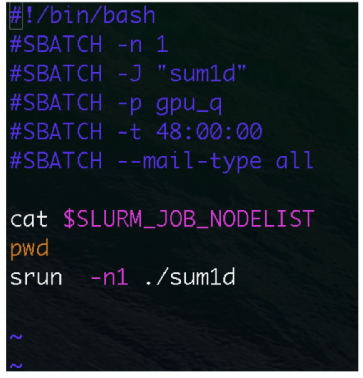
\includegraphics[width=0.6\textwidth, height=0.6\textheight]{script.png}
\end{figure}
\centering{Example of job submission script}
\end{columns}

\end{frame}

\begin{frame}
\frametitle{Use GPU ON the HPC Cluster}
Now let’s submit something to the GPU node of the cluster.\\
\vspace{0.5cm}
Sadly, we have only 1 node (16 CPUs) armed with 2 GPUs\\
\vspace{0.5cm}
Your job has to be submitted to the queue called gpu\_q\\
\vspace{0.5cm}
\ \ \ \ #SBATCH -p gpu\_q\\
\vspace{0.5cm}
The clock limit is 2 days.\\
\vspace{0.5cm}
\ \ \ \ #SBATCH -t 48:00:00\\
\vspace{0.5cm}
\textbf{Goal:} 8 compute nodes with 1 GPU card on each node.
\end{frame}


\begin{frame}
\frametitle{Example: Black-Scholes Option Pricing}

Black-Scholes formula for European options:\\
\begin{eqnarray*}
V_{call} &=& S\Phi(d_1) - X e^{-rT}\Phi(d_2)\\
V_{put} &=&  X e^{-rT}\Phi(-d_2)- S\Phi(d_1)\\
d_1 &=& \frac{log(s/x)+(r+\sigma^2/2)T}{\sigma T}\\
d_2 &=& d_1 - \sigma \sqrt{(T)}\\
\end{eqnarray*}

\textbf{Note:} $\Phi(x)$ is the cumulative standard normal distribution

\end{frame}

\section{Option pricing with GPU}
\begin{frame}
\frametitle{Example: Black-Scholes Option Pricing}

$\Phi(x)$ can be evaluated via numerical approximation 
\begin{eqnarray*}
K &=& \frac{1}{1+0.2316419|d|}\\
\Phi(d) &=& \frac{1}{\sqrt{2\pi}}e^{-d^2/2}[a_1K + a_2 K^2 + a_3 K^3 +a_4K^4 + a_5K^5]\\
a_1 &=& 0.31938153\\
a_2 &=& -0.356563782\\
a_3 &=& 1.781477937\\
a_4 &=& -1.821255978\\
a_5 &=& 1.330274429 
\end{eqnarray*}

\end{frame}

\begin{frame}
\frametitle{Black-Scholes Option Pricing }
The option price $V(S_0, X, T, r, \sigma)$ depends on 5 parameters\\
Set up of the numerical problem.\\
Input parameters:\\
\ \ \ \ S0[4000000] = rand(5, 60)\\
\ \ \ \ X[4000000] = rand(1, 100)\\
\ \ \ \ T[4000000] = rand(1/12, 5)\\
\ \ \ \ r = 0.03\\
\ \ \ \ $\sigma$ = 0.3\\
Output:\\
\ \ \ \ C[4000000]\\
\ \ \ \ P[4000000]\\
Input data S0[],X[], T[] generated on CPU, copied to GPU.\\
Output data C[],P[] calculated by GPU, copied back to CPU.
\end{frame}

\begin{frame}
\frametitle{Black-Scholes Option Pricing}
- Output of computing the 4 million options prices:\\
- Summary: GPU speed up by 267 times is achieved!\\
 \begin{figure}
     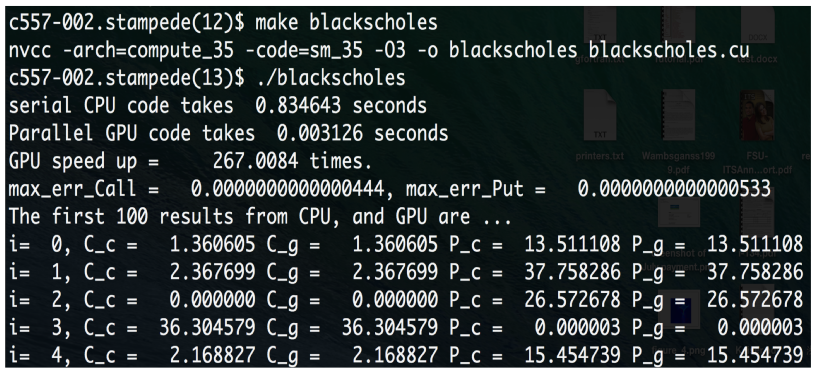
\includegraphics[width=1\textwidth, height=0.6\textheight]{speed.png}
\end{figure}

\centering {GPU VS CPU for Black-Scholes Model} 
\end{frame}

\begin{frame}
\frametitle{Monte-Carlo Option Pricing}
Assume stock price $S(t)$ follows a geometrical Brownian motion.

\begin{columns}
\column{2.4in}
\begin{center}
\begin{equation*}
dS_t = \mu S_t dt + \sigma S_t dW_t\\
dW_t \sim N(0, dt )\\
S(t) = S_0 e ^{\mu t + \sigma \sqrt{t}N(0,1)}\\
\mu = r- 0.5 \sigma^2\\
C(T) = max (S(T) - X, 0 ) 
\end{equation*}
\end{center}
\column{2.5in}
\begin{itemize}
\item $\mu$ is the constant drift.
\item $W(t)$: Wiener process
\item $\sigma$: the volatility
\item $r$: risk free rate
\item $X$: strike price
\item $C(T)$: the option price
\end{itemize}
\end{columns}
\textbf{Goal:} Estimate $C(T)$ by Monte-Carlo simulation of $S(T)$
\end{frame}

\begin{frame}
\frametitle{Monte-Carlo Option Pricing}
What I am going to do is\\
\ \ \ \ Compute option price using the analytical BK formula.\\
\ \ \ \ Estimate option price via Monte-Carlo on CPU (serial).\\
\ \ \ \ Estimate option price via Monte-Carlo on GPU (parallel).\\
\ \ \ \ Compare the performance\\
\vspace{1cm}
About the random number generators\\
\ \ \ \ CPU version: gsl\_ran\_gaussian(). (gnu-science library)\\
\ \ \ \ GPU version: curand\_normal().(cuda random library)\\
\end{frame}

\begin{frame}
\frametitle{Monte-Carlo Option Pricing}
Output of computing the 8192 option prices (131072 paths):\\
Summary: GPU speed up by around 1,000 times!
 \begin{figure}
     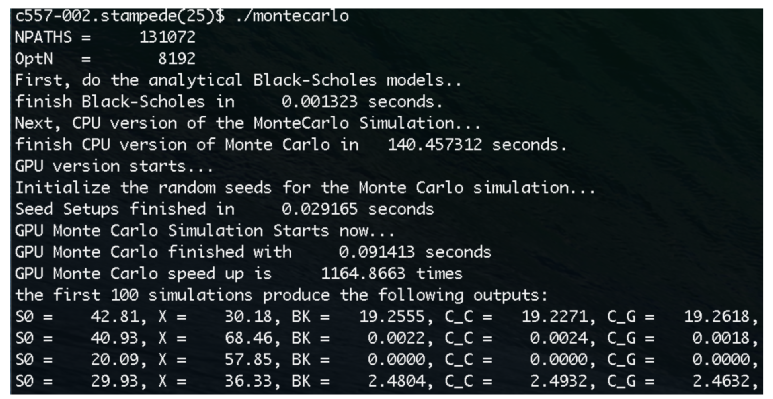
\includegraphics[width=1\textwidth, height=0.6\textheight]{mc.png}
\end{figure}

\centering{GPU VS CPU for Monte-Carlo Option Pricing}


\end{frame}

\begin{frame}
\frametitle{Binomial tree Option Model}
\textbf{Goal:} Price European options using the binomial tree option model.
\begin{columns}
\column{2.4in}
 \begin{figure}
     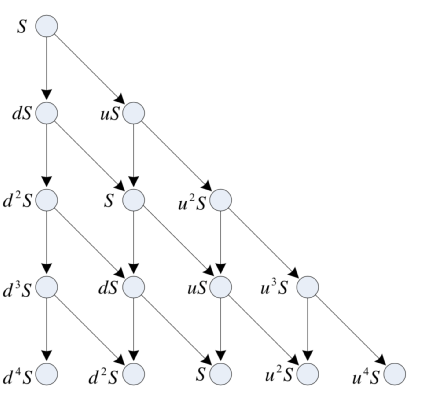
\includegraphics[width=0.8\textwidth, height=0.6\textheight]{binary.png}
\end{figure}
\centering{Binomial tree for 4 time steps}

\column{2.5in}

$$\mu = e^{\sigma \sqrt{dt}}$$\\
$$d = 1/u$$\\
$$P_u =\frac{e^{rd}-d}{u-d}$$\\
$$[P_uu+(1-P_u)d]S_k = S_k s^{rdt}$$

$P_u$ is the probability of pricing going up
\end{columns}

\end{frame}

\begin{frame}
\frametitle{Binomial tree Option Model}
\begin{itemize}
\item Idea: Backward iteration. Let V(t) be price of the option at t.
\item Each node on the tree has exactly two child nodes.
\item The option price on a node can be evaluated using the prices of
its two child nodes.\\
$$V_t = [P_u V_{u, t+dt}+ (1-P_u)V_{d,t+dt}]e^{-rdt}$$
\item The option price on the expiry day, i.e., the leaf node can be
directly evaluated, V = max(S-X, 0).
\item List of parameters {S, X, T, N, r, σ}.
\item Amount of computation of the order O(N*N).
\item In contrast, Black-Scholes work of the order O(1).
\end{itemize}
\end{frame}

\begin{frame}
\frametitle{Binomial tree Option Model}
\begin{itemize}
\item Question: How to realize the iterative algorithm on GPU?
\item At each instant, GPU threads must be working on nodes of the
same level (i.e., same time step).
\item Suppose each thread work on some nodes of the same level,
how to deal with the boundary condition?
\item Each thread has its own number of iteration
 \begin{figure}
     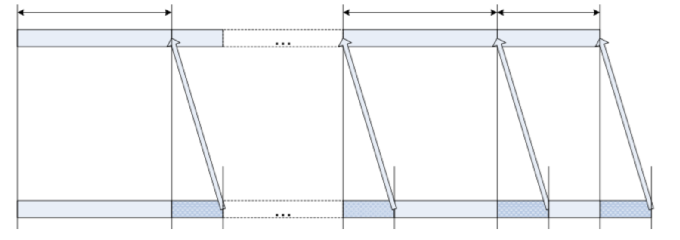
\includegraphics[width=0.8\textwidth, height=0.4\textheight]{split.png}
\end{figure}
\centering{Split work among threads of the block}
\end{itemize}
\end{frame}


\begin{frame}
\frametitle{Binomial tree Option Model}
Numerical set up:\\ 
\ \ \ \ evaluate the price of 1024 options with N = 2048.\\
\ \ \ \ GRIDSIZE = 1024, BLOCKSIZE=128

 \begin{figure}
     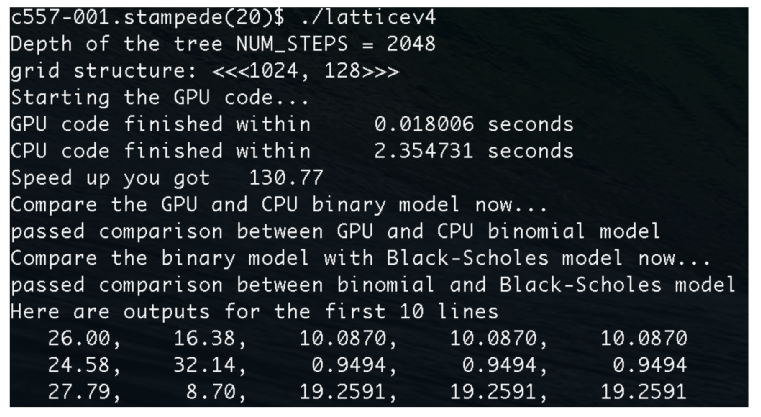
\includegraphics[width=0.8\textwidth, height=0.6\textheight]{binomial.png}
\end{figure}

Results: \alert{130 times} speed up on GPU for binomial tree option model

\end{frame}

\section{Summary}
\begin{frame}
\frametitle{Summary}
\begin{itemize}
\item GPU hardware architecture (why should I care?)
\item CUDA/C/C++ programming model
\item Black-Scholes formula (200x speedup)
\item Monte-Carlo option pricing (1000x speedup)
\item Binomial option model (130x speedup)
\end{itemize}
\end{frame}
\end{document}

